This is a user manual for the desktop client. It will provide guides on how to 
use the client and the different functionalities it holds. The screen shots 
shown in this document are made from a Linux machine, but the application 
also runs on Windows or Mac, and will follow the design principles thereafter. 
Because of this, some details of the look of the client may vary, but the functionality is the same.

\subsection{Login and startup}
When you start this application the first thing that's displayed is a login screen, as illustrated in \refer{fig:des_login-pic}. In this screen you enter your username, password and the IP-Address for the server and then press the login button to enter the \appName\ Desktop.

\begin{figure}[h!]
	\addScaledImage{0.4}{des_login_picture.png}
	\caption{Screenshot of the login screen.}
	\label{fig:des_login-pic}
\end{figure}
The application is built with tabs, as illustrated below in \refer{fig:des_tabs-view}. Each tab contains separate features of the application. There are seven tabs: Search, Upload, Process, Workspace, Administration, Convert and Settings.
\begin{figure}[htb]
	\addImage{des_tabs.png}
	\caption{Illustration of the different tabs of \appName Desktop and displaying the Search tab.}
	\label{fig:des_tabs-view}
\end{figure}
\FloatBarrier

\subsection{Search}
The first tab you see after logging in is the \textit{Search tab}, illustrated in \refer{fig:des_search-query}. The Search tab uses the same query building technique as the \textit{Pubmed Advanced Search Builder}\cite{des_3}. It has one text field where you either can type in the query yourself or you can use the query builder to build the query. \\

To switch between manually editing the query and using the query builder there are two radio buttons to the left of the text field. Each row in the query builder has at most five components. These are a logical expression, an annotation name field, a free text field or a drop down menu to insert search words, a minus button and a plus button. The plus button is only available in the last row and it adda another row to the query. The minus button is used to remove a row and it exists on every row except if there is only one row in the query. The logical expressions combines the annotations, so they are available in every row but the first. \\

By writing in the annotation text field or selecting a value in the drop down menu you can specify the query the row will produce. Together each row builds a full query. As illustrated in \refer{fig:des_search-query} below.
\begin{figure}[htb]
	\addImage{des_search_tab.png}
	\caption{Illustration of a query, made by the query builder.}
	\label{fig:des_search-query}
\end{figure}
\FloatBarrier
\subsubsection{Search results}
When you press the search button the search tab will change it's view to display the search results as illustrated in \refer{fig:des_search-results}. The results are displayed as experiments in a tree table. Each row is an experiment that can be expanded to show more information and the files associated with the experiment. \\

The tree table can be sorted both vertically or horizontally by clicking the headings or by dragging and dropping the columns. You can choose which columns to display by using the menu in the upper right corner of the table. In the same menu there are also buttons for expanding and collapsing all experiments in the search results. \\

To go back to the previous view, you can click the \emph{Back} button. There is also a button called \emph{Add to workspace} for adding the selected files or experiments to the workspace. The last button, \emph{Edit experiment} is used to upload more files to an experiment or to edit information in the marked experiment.

\begin{figure}[htb]
	\addImage{des_search_res.png}
	\caption{Illustration of search results.}
	\label{fig:des_search-results}
\end{figure}
\FloatBarrier

\subsection{Upload}
If you need to upload files to the database it can be done through the upload tab. When the tab is pressed you get presented with a button to create a new experiment shown in figure \ref{fig:des_upload-tab}.

\begin{figure}[h!]
	\addImage{des_upload_tab.png}
	\caption{Illustration of the starting view of the upload tab.}
	\label{fig:des_upload-tab}
\end{figure}
\subsubsection{Existing experiment}
\label{sec:des_exists}
In order to edit files or upload files to an existing experiment you need to search for the experiment in the search tab and then press the \textit{Edit experiment}-button. When this is done the experiment information get retrieved from the server and presented to you. \\

To edit the experiment, change the annotation values and press the \textit{Save changes}-button. To add files to the experiment you can press the button labeled \textit{Browse files}. A file browser window will appear, it is illustrated in figure \ref{fig:des_upload}. Here you can select the files you want to add to the experiment. The files will be added to the upload tab and there will be some new choices available for you. Each file  will be associated with one file row, this is also shown in \ref{fig:des_upload-exists}. \\

The new choices are whether the new files are either raw, region or profile files. And if it is region or profile there is another choice for which genome release. There is also the possiblity to delete the file row, by clicking the \textit{X}-button, in case this file is not suppose to be added to the experiment. When all fields have been filled and the files are correct, you simply click the button labeled \textit{Upload files}. The progress bar will start to progress and if all goes well it will reach 100\% and the files will be added to the existing experiment.

\begin{figure}[h!]
	\addImage{des_upload_existing.png}
	\caption{Illustration of the add to existing experiment part of the upload tab.}
	\label{fig:des_upload-exists}
\end{figure}
\newpage
\subsubsection{New experiment}
\label{sec:des_create}
The first thing you need to do when creating a new experiment (\ref{fig:des_upload-new}) is pressing the button labeled \textit{Create new experiment} in the upload tab. After pressing this button all the different annotations get retrieved from the server. If the annotation is of freetext type there is a textfield to be filled out. If it is a multiple choice annotation there is a drop-down list of the different choices. The annotations who have bold text are forced and needs to be filled out in order to create the experiment. 

In order to add files to this experiment you need to press the \textit{Browse files}-button. A filebrowser will appear and you can choose which files to add. You can also drag and drop files from a folder on your machine onto the upload tab of the client. When the files are added they each get displayed in a file row. The file row consists of the file name and a progress bar. \\

Apart from the add experiments there are also three buttons and a checkbox. The checkbox will be explained in section \ref{sec:des_batch} below. The other three buttons are used in the same manner as in section \ref{sec:des_exists} above. When all the annotations that are needed is filled in and the associated files are added you press the button labeled \textit{Create with all files} to create the experiment.

\begin{figure}[h]
	\addImage{des_upload_new.png}
	\caption{Illustration of the create new experiment part of the upload tab.}
	\label{fig:des_upload-new}
\end{figure}
\subsubsection{Batch upload experiments}
\label{sec:des_batch}
The Genomizer desktop client has support for batch uploading of experiments. The following steps describes how to batch upload experiments:
\begin{enumerate}
	\item Create a new experiment by pressing the button labeled \textit{Create new experiment}.
	\item Press the button labeled \textit{Browse files} and select all the files to be included in the batch upload.
	\item Fill in the experiment ID and annotations of the first experiment
	\item Select one or more files to upload to the first experiment by ticking the check-boxes next to the files.
	\item Select filetype and genome release if needed.
	\item Press the button labeled \textit{Create with selected fiels} and wait for the file(s) to be uploaded. When the upload is complete, the file row will disappear.
	\item When the files have been uploaded, repeat steps 3-6 with the desired changes to annotations and experiment ID's.
	
\end{enumerate}

Using this method let's the user make small changes to annotations while creating multiple experiments.

\begin{figure}[h]
	\addScaledImage{0.5}{des_upload_select.png}
	\caption{Illustration of the file browsing window.}
	\label{fig:des_upload}
\end{figure}
\FloatBarrier


\subsection{Process}
From the \textit{process view} (see \refer{fig:des_process-view}) the user can process files uploaded to experiments. The view consists of three panels; one panel at the top with a drop-down list with process commands, one panel to the left that lists \textit{command components} (see example in \refer{fig:des_rtp-command-component}), and one to the right where feedback from processing tasks can be seen. The top-panel also has a button for adding commands to the list on the left panel.

\begin{figure}[h]
	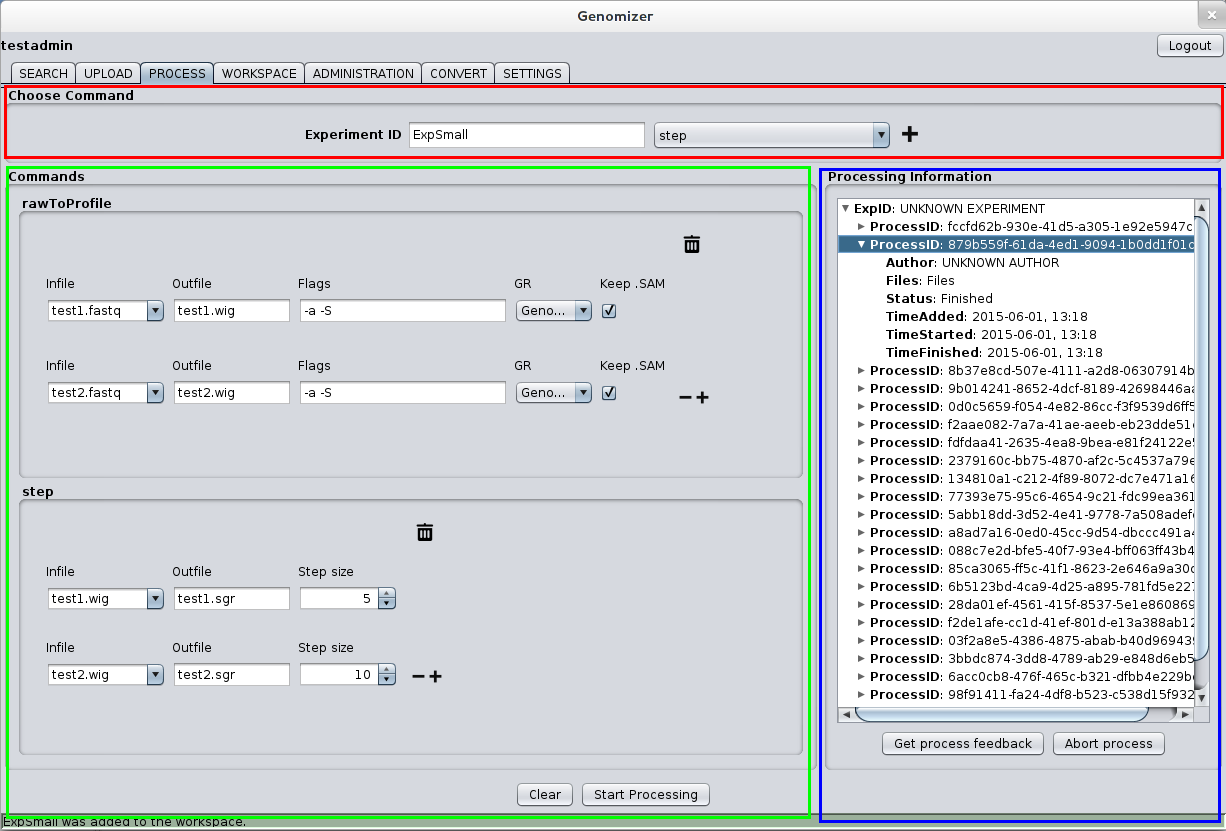
\includegraphics[width=\textwidth, height=\textheight, keepaspectratio]{des_process_view.png}
	\caption{The process view of the Genomizer desktop client. The top-panel (red) has a drop-down list and an add-button. The left panel (green) lists process commands to be performed in the processing sequence. The right panel (blue) shows the status of different processing tasks.}
	\label{fig:des_process-view}
\end{figure}

\begin{figure}[h]
	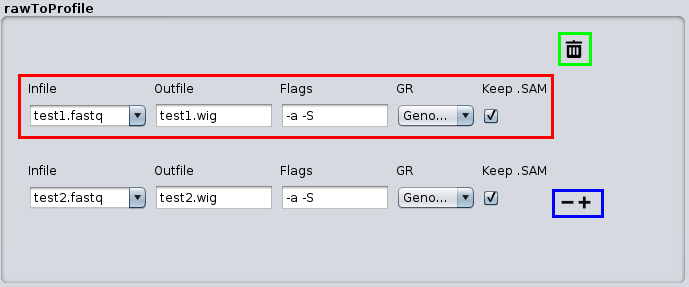
\includegraphics[width=\textwidth, height=\textheight, keepaspectratio]{des_rtp_command_component.png}
	\caption{A command component representing a raw-to-profile-process. The component has rows for input parameters (red), buttons to add and remove input rows (blue), and a button to remove the entire component (green).}
	\label{fig:des_rtp-command-component}
\end{figure}

To prepare an experiment for processing the following steps must be performed:
\begin{itemize}
	\item Search for the desired experiment and add it to the workspace, as described under the search section.
	\item Select the experiment from the worksapce view and press the button labeled 	\textit{Process}.
\end{itemize}
After performing these steps, the user can process the files of the selected experiment. The user can perform several process steps in a sequence, and also perform each step on several files. A command component in the list on the left panel represents a step in the processing sequence. Each command component has a row for input fields, where the user can select files to apply the command on, specify names of resulting files, and define other parameters. The command component also have buttons for adding and removing extra input-rows, and a button for removing the whole component.

The following describes how to process one or more files:
\begin{itemize}
	\item Select a process command from the drop-down list located on the top-panel of the tab.
	\item Click the plus-button next to the drop-down list to add the command to the command list located below.
	\item In the command component in the list, fill in the needed parameters. Click the plus-button on the command component to add more files to process, or remove unwanted files by pressing the minus-button.
	\item To add another command to the sequence, repeat the above steps.
	\item To remove undesired commands, press the trash can icon in the upper-right corner of the command component. To remove all commands press the button labeled \textit{Clear}.
	\item When the desired process commands have been added and parameters have been filled in, press the button labeled \textit{Start Processing} to start processing.
\end{itemize}	
	The server will now start processing the specified files with the specified commands and parameters, in the same order the commands were added by the user. To get feedback from the processing task, the user can press the button labeled \textit{Get process feedback}. To abort ongoing process tasks, the user can press the button labeled \textit{Abort process}. The feedback panel lists experiments, which can be expanded to show the status of processing tasks, associated with the expanded experiment.

\FloatBarrier

\subsection{Workspace} \label{sec:des_workspace}
The workspace Tab seen in \refer{fig:des_workspace-view} is a tab where you can temporarily store experiments and their files, and choose different options for action. Results from various searches can be stored here, and the contents of the workspace is saved as long as the program is running. Files and/or experiments are chosen by clicking them, multiple files by using either Shift-click, Ctrl-click or simply holding down the mouse button and dragging the cursor over multiple files. By choosing an experiment, all of the containing files are selected.
\subsubsection{Delete from workspace}
Items can be deleted from the Workspace by pressing \textit{Remove from workspace}.
\subsubsection{Delete from database}
To delete the selected data from the database the \textit{Delete from database} button should be used instead. When pressing the delete button a small popup window with a progress bar will be displayed. By closing this window the deletion of data can be aborted.
\subsubsection{Upload to}
If you want to upload files to an experiment you have in the workspace, you can simply click the \textit{Upload to} button to switch to the upload tab and upload to the experiment they have selected. If multiple experiments have been selected, only the first one will be uploaded to.
\subsubsection{Process}
If you want to add files to the process tab there is a \textit{Process} button which transfers the selected experiment to the process tab.
\subsubsection{Download}
You can make the choice to download files to their local computer. If you press the \emph{Download} button seen in \refer{fig:des_workspace-view}, you get to choose a directory where you want to save the files. When a directory has been chosen, the files get downloaded and all current and completed download can be seen in the tab \emph{downloads}, see \refer{fig:des_download-view}.
\begin{figure}[htb]
	\addImage{des_workspace_select.png}
	\caption{Screenshot of the workspace tab in the program.}
	\label{fig:des_workspace-view}
\end{figure}
\begin{figure}[htb]
	\addImage{des_download.png}
	\caption{The downloads tab of the workspace}
	\label{fig:des_download-view}
\end{figure}
\FloatBarrier

%SYSADMIN START HERE...!
\subsection{Administration}
\subsubsection{annotation}

The system administration tools for the desktop client is available under the Administration tab. There are two different tools: Annotation and Genome files. The annotation tab is the first sub tab in the Administration tab. Annotations are used for specifying properties of uploaded data. For example, if new data from an experiment done with rat tissue is uploaded, the data shuld have an annotation called "species" with the value "rat". The Annotations sub tab in the Administration tab gives you the tools to create, edit and remove annotations and annotation values. 
\begin{figure}[htb]
	\addImage{annotationsView.png}
	\caption{The annotation view}
	\label{fig:annotationsView}
\end{figure}

In the annotations tab, when you press the button labeled \textit{Add} in the sidepanel a new popup window appears. It is possible to write the name of the new annotation and the new values in this popup, as well as check a "forced annotation"-box. The "forced" value determines if the annotation will have to be present in all future file uploads. See \refer{fig:adm_addAnnotationPopup}

\begin{figure}[htb]
	\addScaledImage{0.6}{adm_addAnnotationPop.png}
	\caption{The add annotation popup}
	\label{fig:adm_addAnnotationPopup}
\end{figure}

If you want to have free text as a value, for example if the annotation is pubmedID, the value of that annotation will not be able to be chosen from a drop-down menu, since the number available values is enormous. You might then want to use a freetext annotation, which allows you to type any value you want. To create a freetext annotation you click on the freetext tab on the "add" popup. 


To remove an annotation, you select an annotation from the table in the center of the view, and click on the remove button on the right side. You then have to confirm this deletion. After this the annotation is completely removed and cannot be brought back to life, see \refer{fig:adm_desktopRemoveAnnotation}. Some annotations cannot be removed for security reasons, 'Species' is such an annotation. Trying to remove it will generate an error message.
\begin{figure}[h!]
\addImage{adm_removeAnnotation.png}
\caption{The remove annotation popup.}
\label{fig:adm_desktopRemoveAnnotation}
\end{figure}
\subsubsection{Genome files}


The genome files tab shown in \refer{fig:adm_desktopGenomeTab} contains a table with information about which genome release versions are stored on the server. If you click on one of the entries, a smaller frame is displayed at the bottom of the table showing which files are included in the selected genome release. To the right of the genome release tab are the tools for adding new genome releases. You can name the new genome release in the text field and you are then able to upload the files associated with that genome release. \\

When the desired files are selected, progress bars representing the upload of those files appear at the bottom of the \textit{Add Genome Release}-frame. When you press the button labeled \textit{Upload}, the upload of the selected files will start and you can follow the upload progress from the progress bars. After the upload is finished, you will be notified of its success or failure with a message dialog.
Genome releases can also be removed by selecting the release version from the table and pressing the \textit{Remove genome release}-button which appears at the bottom of the table when a release version is selected. This will remove the genome release and all associated files.

\begin{figure}[h!]
\addImage{genomeReleaseViewExtraInfo.png}
\caption{The genome release view.}
\label{fig:adm_desktopGenomeTab}
\end{figure}

If you want to add a new species to add or remove genome releases for, this can be done in the top right corner of the genome release tab. You simply writes the name of the new species and presses the \textit{add}-button and the species will be added to the "Species" annotation.


\subsubsection{Users}

The Users tab shown in \refer{fig:des_users} contains four different panels, one to create a new user, one to update an existing user, one to delete an existing user and one to show all the users. Just fill in all information in the text fields and press one of the buttons to do that command. There is three different kind of users, the Guest, User and the admin. The Admin is the only one to have access to this User tab.


 \begin{figure}[h!]
 \addImage{des_users.png}
 \caption{The Users admin view.}
 \label{fig:des_users}
 \end{figure}


\subsection{Convert}

The Convert tab shown in \refer{fig:des_convert} contains buttons to convert and remove selected files, and buttons to choose what to convert into. The panel \textit{Convert from} shows the files sent into the convert tab, and the panel \textit{Converted files} shows the finished files that have been converted. \\

To convert files, begin with selecting the wished files to convert in the \refer{fig:des_workspace-view} and press the convert button. You will be directed to the convert tab with the files, check all the files you want to convert (only possible to convert one filetype at a time) and press the \textit{Convert selected files}-button. If the files managed to convert successfully they will appear in the \textit{Converted files}-panel  to the right. \\

Notice that you need to choose which filetype you want to convert into in the \textit{Convert to}-panel if the selected files can be converted into many different filetypes. The convert from panel is only in the panel for show, to show which filetypes you have selected. \\

Remove files from the list by pressing the \textit{Remove selected files}-button, and clear the list with finished conversions by clicking on the \textit{Clear converted files}- button.


 \begin{figure}[h!]
 \addImage{des_convert.png}
 \caption{The Convert tab.}
 \label{fig:des_convert}
 \end{figure}

\subsection{Settings}

In the settings tab \refer{fig:des_settings} you can change password and information about your user. To change information, all fields must be filled. When the fields are filled, press the update settings.

 \begin{figure}[h!]
 \addImage{des_settings.png}
 \caption{The Settings tab.}
 \label{fig:des_settings}
 \end{figure}
